\chapter{Aprendizado por reforço}

\framebox[\textwidth]{
	\hspace{1em}
	\vbox{
		\textbf{Leitura obrigatória:}
		\begin{itemize}
			\item \cite{RusselAndNorvig2010} -- Cap. 21 (Aprendizagem por reforço).
			\item \cite{Mitchell1997} -- Cap. 13 (Reinforcement Learning).
		\end{itemize}
		
		\textbf{Leitura complementar:}
		\begin{itemize}
			\item \cite{SuttonAndBarto1998} -- Cap. 1 (Introduction).
			\item \cite{SuttonAndBarto1998} -- Cap. 3 (The Reinforcement Learning Problem).
		\end{itemize}
	}
}

\section{Visão geral}

O aprendizado por reforço tem por objetivo fazer com que um agente aprenda a forma como deve agir para execução de alguma tarefa. O agente aprende a escolher a ação ótima através da sua interação com o ambiente. Por exemplo, um agente pode aprender a movimentar-se em um ambiente físico, organizar volumes em um estoque, ou ainda jogar algum jogo de tabuleiro.

Para isso, o aprendizado por reforço considera que o ambiente (ou um supervisor externo) forneça um retorno ao agente quando ele atinge o objetivo ou quando atinge algum estado de fracasso. O agente recebe uma recompensa (positiva ou negativa) conforme as ações executadas e, com isso, aprende a sequência de ações que maximiza a recompensa. Por exemplo, treinar um agente para jogar damas consiste em dar uma recompensa positiva caso ele ganhe o jogo, uma recompensa negativa caso ele perca o jogo, e nenhuma recompensa nos estágios intermediários. Com isso, o agente aprende a sequência de ações que o levam à vitória e, dessa forma, aprende a jogar damas.

\begin{figure}
	\centering
	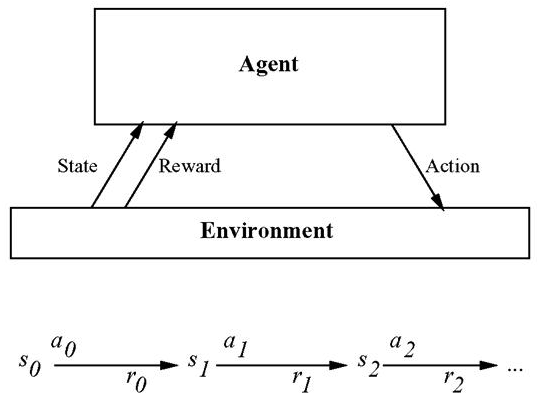
\includegraphics[width=0.5\textwidth]{img/agente-ambiente-recompensa}
	\caption{Interação entre agente e ambiente com recompensa pelas ações}
	\label{fig:agente-ambiente-recompensa}
\end{figure}

A Figura~\ref{fig:agente-ambiente-recompensa} apresenta a ideia geral onde o agente, além de perceber o ambiente e agir sobre ele, recebe uma recompensa em função da ação executada e do resultado obtido por ela. A figura ainda mostra os elementos principais do aprendizado por reforço. Dado um estado $s_0$, o agente executa a ação $a_0$, que modifica o ambiente para o estado $s_1$. Com isso, o agente recebe a recompensa $r_0$. O mesmo ocorre quando, a partir do estado $s_1$, o agente executa a ação $a_1$, levando-o para o estado $s_2$ e recebendo a recompensa $r_1$. Neste sentido, a tarefa do agente é aprender a sequência de ações que maximize as recompensas obtidas. Logo, o aprendizado por reforço torna-se bastante abrangente, podendo ser aplicado a uma variedade de problemas de aprendizagem.

A sequência de ações que o agente deve aprender é chamada de \textbf{política} (ou política de controle). A política é, portanto, uma função que mapeia estados para ações. Podemos denotar a política como $\pi : S \rightarrow A$, que retorna uma ação $a \in A$, dado um estado $s \in S$. Uma notação igualmente comum é $a = \pi(s)$.

O aprendizado por reforço possui algumas características que o difere de outras técnicas de aprendizagem de máquina:

\begin{itemize}
	\item \textbf{Recompensa tardia:} em outras tarefas de aprendizagem de máquina, o agente possui um conjunto de dados de treinamento, sobre o qual deve induzir uma hipótese. No aprendizado por reforço, não existem dados rotulados ou disponíveis \textit{a priori}. O agente deve explorar o conjunto possível de ações e, com o retorno recebido, aprender a política ótima.
	
	\item \textbf{Exploração:} para conhecer as diferentes possibilidades de ações e transições de estados, bem como descobrir qual a melhor sequência de ações, o agente deve explorar o ambiente. Com isso, o agente deve preocupar-se com o equilíbrio entre \textit{explorar} ações desconhecidas, ou \textit{intensificar} sua busca nos melhores caminhos de ações já encontrados (exploração $\times$ intensificação).
	
	\item \textbf{Estados parcialmente observáveis:} muitas vezes o agente não possui a visão completa do seu ambiente. Neste caso, é comum que a melhor ação a se tomar seja aquela que permita uma percepção mais abrangente do seu ambiente. Como exemplo, considere um robô cuja câmera consiga captar apenas parte do entorno.
	
	\item \textbf{Aprendizado de vida longa:} diferente de tarefas de predição de uma função isolada, um agente físico deve aprender atividades periféricas como recarregar sua bateria, movimentar-se para chegar a um ponto específico, etc. Uma vez que o agente pode aprender a partir da exploração do ambiente, não se faz necessária a manutenção de um grande conjunto de dados de teste.
\end{itemize}

\section{Processo de decisão de Markov}

O Processo de Decisão de Markov (MDP -- \textit{Markov Decision Process}) é aplicado quando se deseja tomar uma sequência de decisões, mas o resultado de cada decisão não é claro. O MDP permite, matematicamente, determinar uma política que maximize o retorno esperado da sequência de decisões. Neste sentido, a tarefa de aprendizagem por reforço pode ser modelada como um MDP.

\subsection{Funcionamento}

Em cada instance discreto de tempo $t$, o agente percebe o estado atual $s_t$, escolhe e executa a ação atual $a_t$. O ambiente responde com uma recompensa $r_t = (s_t, a_t)$ e produz o estado sucessor $s_{t+1} = \delta(s_t, a_t)$. As funções $r$ e $\delta$ fazem parte do ambiente e não necessariamente são conhecidas pelo agente\footnote{Em muitos casos, estas funções podem ser implementadas diretamente no agente.}.

Queremos aprender uma política ótima $\pi(s_t) = a_t$ em que dado um estado $s_t$, o agente possa escolher a melhor ação possível $a_t$. A política ótima é aquela que produz a maior recompensa acumulada. Logo, podemos definir a recompensa acumulada como:

\begin{align*}
V^\pi(s_t) &\equiv r_t + \gamma r_{t+1} + \gamma^2 r_{t+2} + \hdots \\[10pt]
&\equiv \sum_{i=0}^{\infty} \gamma^i r_{t+i}
\end{align*}

A constance $0 \le \gamma < 1$ determina o valor relativo entre recompensas a serem recebidas no futuro e a recompensa imediata. Ou seja, uma recompensa recebida $i$ passos a frente é descontada exponencialmente por um fator $\gamma^i$. Se definirmos $\gamma = 0$, somente a recompensa imediata é considerada. Por outro lado, com $\gamma$ próximo a 1 é dada maior ênfase a recompensas futuras em relação à recompensa imediata. Logo, $V^\pi(s)$ pode ser chamada de \textit{recompensa cumulativa descontada} obtida pela política $\pi$ a partir do estado $s$.

Com isso, a tarefa de aprendizado do agente consiste em selecionar a política que maximiza a recompensa cumulativa descontada para todos os estados. Chamamos esta política de \textbf{política ótima} e denotamos por $\pi^*$. A recompensa cumulativa descontada da política ótima $V^{\pi^*}(s)$ pode ser simplificada para $V^*(s)$. Com isso, denotamos a política ótima como:

$$
\pi^* \equiv \argmax_{\pi} V^\pi(s), \forall s
$$

\subsection{Exemplo -- movimentação no ambiente de grade}

Consideremos o ambiente apresentado na Figura~\ref{fig:exemplo-rl-cenario}. Consiste em uma grade em que cada célula representa um possível estado. As setas representam as possíveis ações de movimentação do agente, cujo valor associado corresponde à recompensa da respectiva ação. Perceba que o estado \textbf{G} é o único que atribui uma recompensa diferente de zero às ações que levam a ele. Logo, podemos chamá-lo de \textit{estado objetivo}. Além disso, ele não possui ações que permitam ao agente sair deste estado, o que nos permite chamá-lo de \textit{estado de absorção}. A tarefa, portanto, consiste em determinar a sequência de ações que levam ao estado objetivo pelo menor caminho.

\begin{figure}[h]
	\centering
	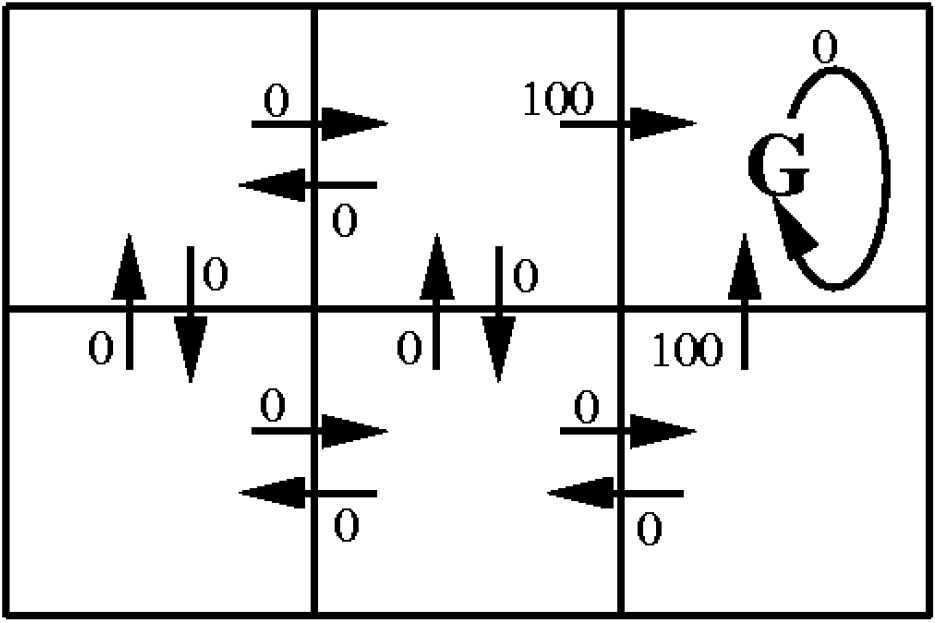
\includegraphics[width=0.3\textwidth]{img/exemplo-rl-cenario}
	\caption{Ambiente em grade cuja tarefa é chegar ao estado G}
	\label{fig:exemplo-rl-cenario}
\end{figure}

Uma vez definidos os estados, ações e recompensas, precisamos definir o valor do desconto $\gamma$ para definir a política ótima $\pi^*$. Consideremos $\gamma = 0.9$. A Figura~\ref{fig:exemplo-rl-politica-otima} mostra uma política ótima (podem existir outras) para este cenário. Esta política move o agente diretamente para o estado objetivo, considerando o menor número de passos possível. Como qualquer política, ela define uma única possível ação a partir de um determinado estado.

\begin{figure}[h]
	\centering
	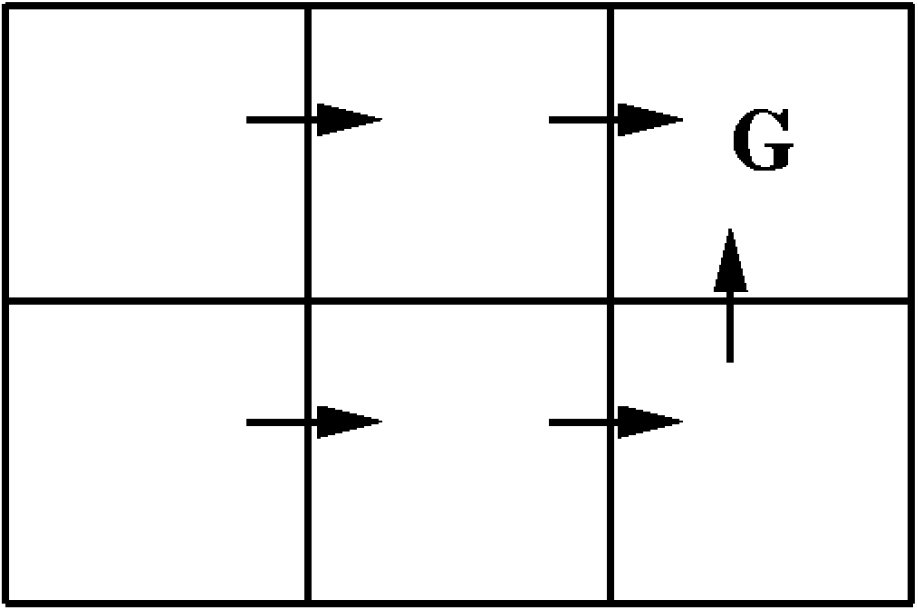
\includegraphics[width=0.3\textwidth]{img/exemplo-rl-politica-otima}
	\caption{Uma política ótima para o ambiente em grade}
	\label{fig:exemplo-rl-politica-otima}
\end{figure}

A Figura~\ref{fig:exemplo-rl-recompensas} mostra o ambiente em grade preenchido com os valores de recompensa $V^*(s)$ para cada estado, considerando o fator de desconto $\gamma = 0.9$. O estado inferior direito possui valor associado de recompensa 100 pois selecionando a ação ``\textit{para cima}'' o agente receberá uma recompensa \textit{imediata} de 100. O mesmo acontece com o estado a esquerda do estado \textbf{G}. Já o estado inferior central possui recompensa de 90, pois a ação ``\textit{para direita}'' não leva a uma recompensa imediata. Logo, a recompensa futura deve ser descontada. Aplicando o fator de desconto $\gamma^1$, pois a recompensa será recebida 1 passo no futuro, associamos a recompensa resultante ($0.9 \times 100 = 90$) a este estado. O mesmo acontece com o estado inferior esquerdo, a recompensa está dois passos a frente, logo utilizamos o fator de desconto $\gamma^2 = 0.81$ e associamos a recompensa $0.81 \times 100 = 81$ a este estado.

\begin{figure}[h]
	\centering
	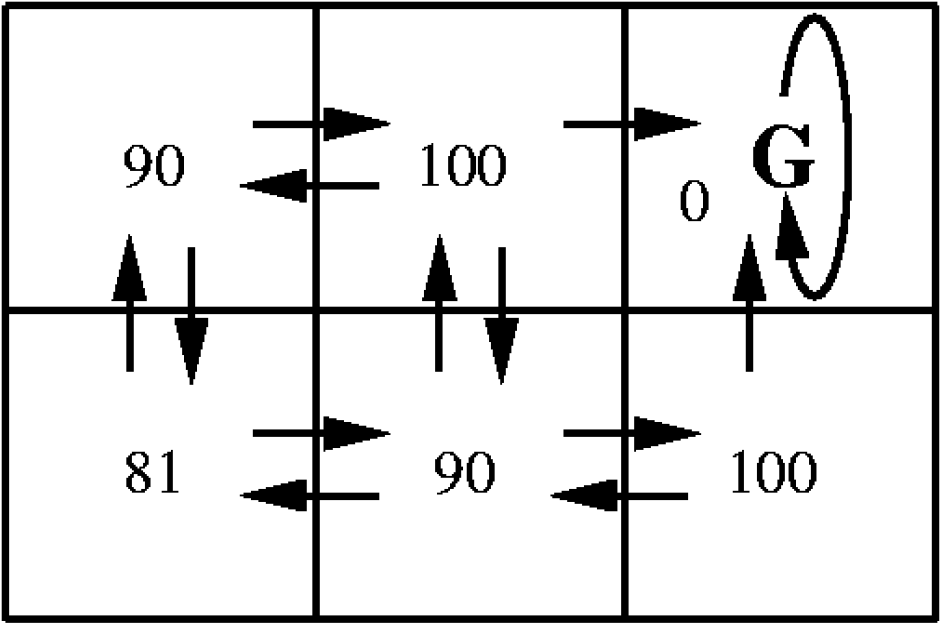
\includegraphics[width=0.3\textwidth]{img/exemplo-rl-recompensas}
	\caption{Valores de recompensa $V^*(s)$ da política ótima para o ambiente em grade}
	\label{fig:exemplo-rl-recompensas}
\end{figure}

\section{Algoritmo de \textit{Q}-Learning}

O algoritmo de $Q$-Learning é a abordagem mais conhecida de aprendizado por reforço. Esta seção mostra seu funcionamento, aplicação e um exemplo.

\subsection{Funcionamento}

O Algoritmo de $Q$-Learning permite ao agente aprender uma política ótima $\pi^*$ para qualquer ambiente arbitrário. A cada estado, o agente deve selecionar a ação $a$ que forneça o maior benefício em termos da recompensa imediata $r(s, a)$ somada à recompensa futura acumulada do próximo estado $V^*(s')$, descontado por $\gamma$. Considerando que o próximo estado é obtido em função da execução da ação $a$ no estado atual $s$, temos $s' = \delta(s, a)$. Com isso, definimos a função $Q$ (que dá nome ao algoritmo), como a maior recompensa acumulada descontada que pode ser obtida a partir do estado $s$, aplicando a ação $a$ como primeira ação.

$$
Q(s, a) = r(s, a) + \gamma V^* (\delta(s, a))
$$

A função $Q$ pode ainda ser vista como a recompensa obtida pela execução de $a$ em $s$, mais a recompensa descontada ao seguir a política ótima após isso. Como o agente seleciona a ação que maximiza $Q(s, a)$, a política ótima é definida por:

$$
\pi^*(s) = \argmax_{a} Q(s, a)
$$

Se o agente conhece as funções $r(s, a)$ e $\delta(s, a)$, isto é, ele possui conhecimento completo do ambiente, ele pode determinar o valor de $Q$ para todas as ações e, com isso, obter a política ótima. A Figura~\ref{fig:exemplo-rl-tabela-q} apresenta o valor de $Q$ para todas as ações possíveis. Perceba que ao selecionar a ação que maximiza $Q$ em cada estado, chegamos ao estado objetivo com o menor número de passos possível.

\begin{figure}[h]
	\centering
	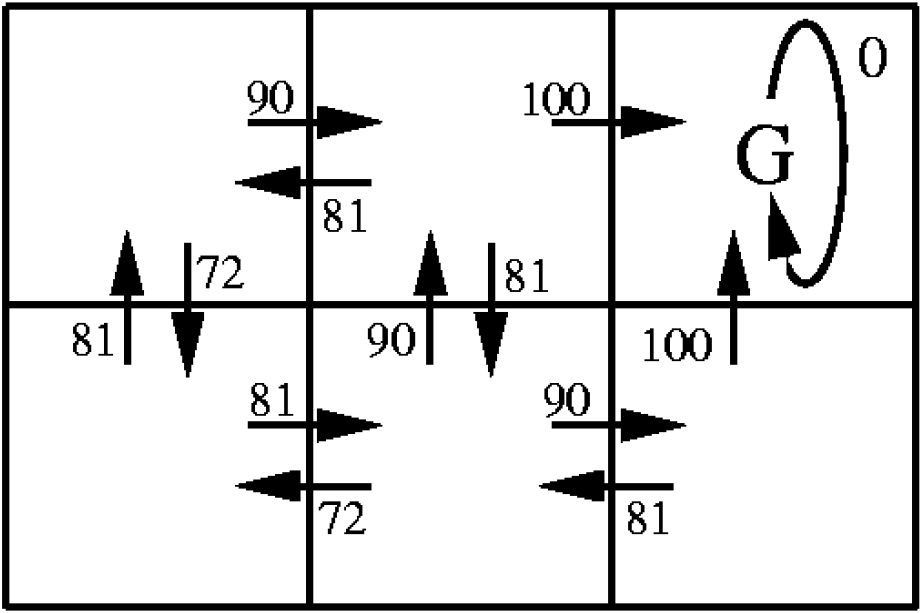
\includegraphics[width=0.3\textwidth]{img/exemplo-rl-tabela-q}
	\caption{Valores de $Q(s, a)$ para o ambiente em grade}
	\label{fig:exemplo-rl-tabela-q}
\end{figure}

É correto afirmar que a recompensa acumulada descontada $V^*(s)$ é igual à maximização da função $Q$, para um dado estado. Ou seja:

$$
V^*(s) = \max_{a'} Q(s, a')
$$

Com isso, podemos reescrever a função $Q$ como uma recursão da seguinte forma:

$$
Q(s, a) = r(s, a) + \gamma \max_{a'} Q(\delta(s, a), a')
$$

O agente deve induzir uma hipótese para a função $Q$. A hipótese induzida é representada por $\widehat{Q}$. O agente representa esta hipótese através de uma grande tabela, contendo o valor associado a cada par \textit{estado-ação}. Ou seja, a entrada $\langle s, a \rangle$ armazena o valor de $\widehat{Q}(s, a)$\footnote{Perceba que não se trata do valor real $Q(s, a)$, mas da indução do agente sobre este valor.}. O agente inicializa esta tabela com zero (ou outros valores aleatórios) e repetidamente observa seu estado atual $s$, seleciona uma ação $a$, executa a ação e observa a recompensa $r = r(s, a)$ e o novo estado $s'= \delta(s, a)$. Após isso, ele atualiza a entrada da tabela $\widehat{Q}(s, a)$ seguindo a regra:

$$
\widehat{Q}(s, a) \gets r + \gamma \max_{a'} \widehat{Q}(s', a')
$$

Perceba que a atualização da tabela utiliza os próprios valores previamente armazenados ($\widehat{Q}$). Com isso, o agente não precisa conhecer as funções $\delta$ e $r$ para aprender, basta repetidamente explorar o ambiente, verificando o estado e a recompensa resultante da ação executada e, com isso, atualizar a tabela $\widehat{Q}$. Portanto, $\widehat{Q}$ pode ser visto como uma aproximação da função real $Q$.

O Algoritmo~\ref{alg:q-learning} apresenta um pseudocódigo para o algoritmo de $Q$-Learning. O primeiro passo consiste em inicializar a tabela $\widehat{Q}$. Após isso, repetidamente o agente percebe seu estado inicial e, enquanto não encontrar o estado objetivo ele seleciona uma ação, a executa, verifica a recompensa imediata e o estado resultante, atualizando a tabela $Q$. Este processo é repetido por um conjunto finito de iterações, chamadas de \textbf{episódios}. A quantidade de episódios é determinada pelo parâmetro $e$. Ao final, o agente aproxima a política ótima, que é armazenada na tabela $\widehat{Q}$.

\begin{algorithm}[h]
	\DontPrintSemicolon
	\Entrada{\textit{fator de desconto} -- $\gamma$; \textit{número de episódios} -- $e$}
	\Saida{\textit{agente aprende um comportamento}}
	
	\Inicio{
		\Para{cada par $\langle s, a \rangle$}{
			Inicializa a entrada da tabela $\widehat{Q}(s, a)$ com zero\;
		}
		Observa o estado atual $s$\;
		
		\Enqto{$e > 0$}{
			\Enqto{$s$ não é o estado objetivo}{
				Seleciona uma ação $a$ e a executa\;
				Recebe a recompensa imediata $r$\;
				Observa o novo estado resultante $s'$\;
				Atualiza a entrada da tabela: $\widehat{Q}(s, a) \gets r + \gamma \max_{a'} \widehat{Q}(s', a')$\;
				$s \gets s'$\;
			}
			$e \gets e - 1$\;
		}
	}
	
	\caption{Pseudocódigo para o algoritmo $Q$-Learning}
	\label{alg:q-learning}
\end{algorithm}

A estratégia de escolha da ação $a$ (linha 7) é fundamental na implementação do algoritmo $Q$-Learning. Se sempre escolhermos a melhor ação conhecida, podemos descartar sequências de ações melhores, porém desconhecidas. É importante definirmos um comportamento exploratório, combinado com a intensificação das melhores ações conhecidas (exploração $\times$ intensificação).

A abordagem gulosa sempre escolhe a melhor ação possível. Para evitar a convergência para uma política ruim, a estratégia $\epsilon$-gulosa propõe selecionar uma ação aleatória com probabilidade $\epsilon$, e selecionar a melhor ação conhecida com probabilidade $1 - \epsilon$ (neste caso, $\epsilon$ é um parâmetro de entrada do algoritmo). Finalmente, uma prática comum é atualizar o valor de $\epsilon$ com o passar do tempo, mantendo um comportamento mais exploratório no início e menos exploratório a medida que os episódios são executados. Por exemplo, pode-se iniciar com $\epsilon = 1$ (totalmente aleatório) e, a cada episódio, multiplicar $\epsilon$ por $0,95$.

Outras estratégias são:
\begin{itemize}
	\item A cada episódio fazer com que o agente inicie em um estado diferente, fazendo com que ele explore diferentes situações. Nem todos os problemas permitem a aplicação desta estratégia.
	
	\item Limitar o número máximo de passos para o agente cumprir a tarefa. Caso ele não obtenha sucesso após o número máximo de passos, ele reinicia o processo (próximo episódio).
\end{itemize}

\subsection{Exemplo -- encontrar a moeda em um cenário em grade}

Vamos considerar um agente que se movimenta em um ambiente em grade com o objetivo de coletar uma moeda. O ambiente é apresentado na Figura~\ref{fig:exemplo-moeda-q-learning}, sendo composto por nove células e, portanto, nove estados. Cada estado é identificado por uma letra: $A, B, \hdots, I$. O agente pode iniciar em qualquer posição do ambiente (por exemplo: $A$) e a moeda possui uma posição fixa ($I$). O agente deve aprender a movimentar-se no sistema para coletar a moeda com o menor número possível de passos.

\begin{figure}[h]
	\centering
	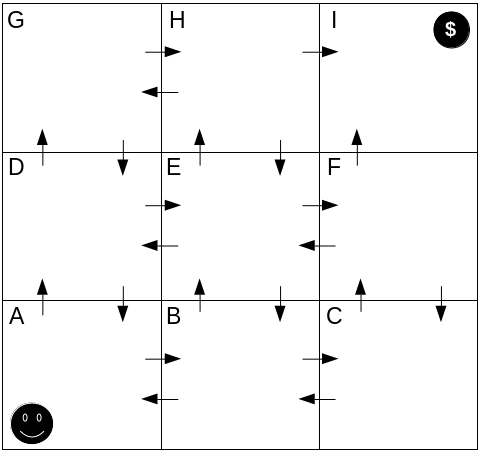
\includegraphics[width=0.45\textwidth]{img/exemplo-moeda-q-learning-1}
	\caption{Cenário da moeda na sua situação inicial}
	\label{fig:exemplo-moeda-q-learning}
\end{figure}

Para implementar o algoritmo de aprendizado por reforço para este agente, devemos definir o esquema de recompensas que o agente recebe, a estratégia com a qual o agente seleciona uma ação e o fator de desconto.
\begin{itemize}
	\item \textbf{Recompensas:} ao chegar no estado onde encontra-se a moeda, o agente recebe uma recompensa de 100. Nos demais estados o agente não recebe recompensa (ou seja, recebe 0). Consideremos ainda $I$ como o estado final e um estado de absorção.
	\item \textbf{Seleção de ações:} estratégia $\epsilon$-gulosa com $\epsilon = 0.2$.
	\item \textbf{Fator de desconto:} consideremos $\gamma = 0.9$.
\end{itemize}
.
Inicialmente, todas as entradas da tabela $\widehat{Q}(s, a)$ são inicializadas com zero, conforme a situação apresentada na Figura~\ref{fig:exemplo-moeda-q-learning}, em que nenhuma seta (ação) possui valor atribuído. Neste caso, todas as ações possuem recompensa esperada de zero, o que faz com que o agente selecione qualquer ação em qualquer estado que se encontre. Suponha que o agente selecione aleatoriamente a ação $A \rightarrow B$. Isso faz com que o agente receba recompensa imediata $r = 0$. A entrada correspondente da tabela $\widehat{Q}$ é atualizada conforme:

$$
\widehat{Q}(s, a) \gets r + \gamma \max_{a'} \widehat{Q}(s', a')
$$

Neste caso, $r = 0$ (recompensa imediata). Dado o novo estado $s' = B$, o agente deve verificar a melhor ação possível a partir de $B$ e somar a sua recompensa esperada, aplicando o desconto $\gamma$. A partir do estado $B$, todas as ações possuem recompensa esperada igual a 0. Logo, a entrada $\widehat{Q}(A, A \rightarrow B)$ permanece com o valor 0. Isso se repete enquanto o agente se movimenta no ambiente sem receber uma recompensa. Por exemplo, o agente poderia fazer o caminho $A \rightarrow B \rightarrow E \rightarrow D \rightarrow E \rightarrow H$. Ao selecionar uma ação que leva ao estado $I$ (por exemplo, $H \rightarrow I$), o agente recebe uma recompensa imediata $r = 100$. A recompensa futura esperada é 0, pois $I$ é um estado de absorção. Logo, $\widehat{Q}(H, H \rightarrow I) = 100$. Com isso, o primeiro episódio termina e a Figura~\ref{fig:exemplo-moeda-q-learning-2} apresenta o ambiente com os valores de recompensa atualizados.

\begin{figure}[h]
	\centering
	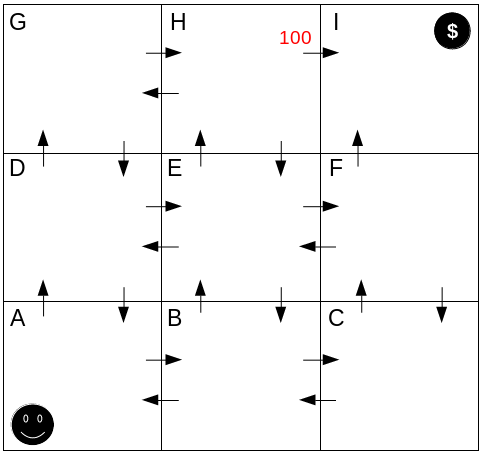
\includegraphics[width=0.44\textwidth]{img/exemplo-moeda-q-learning-2}
	\caption{Cenário da moeda ao encontrar o estado objetivo a partir de $H$}
	\label{fig:exemplo-moeda-q-learning-2}
\end{figure}

No segundo episódio, novamente o agente inicia no estado $A$ e não sabe qual a melhor ação a ser tomada, escolhendo aleatoriamente entre as ações disponíveis. Porém, suponhamos que o agente chegue no estado $G$ e selecione a ação $G \rightarrow H$. Neste caso, ele recebe uma recompensa imediata igual a 0, mas ao computar a recompensa futura, ele sabe que a partir de $H$ ele pode chegar a um estado com recompensa 100. Ou seja, $\max_{a'} \widehat{Q}(H, H \rightarrow I) = 100$. Logo, $\widehat{Q}(G, G \rightarrow H) = 0 + 0.9 \times 100 = 90$. Com isso, ao final do segundo episódio temos a situação apresentada na Figura~\ref{fig:exemplo-moeda-q-learning-3}.

\begin{figure}[h]
	\centering
	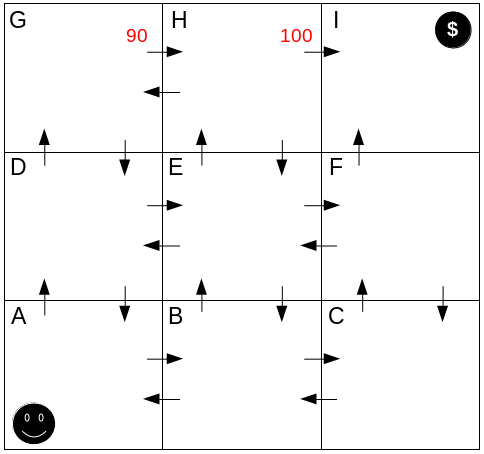
\includegraphics[width=0.44\textwidth]{img/exemplo-moeda-q-learning-3}
	\caption{Cenário da moeda ao encontrar um estado com recompensa futura}
	\label{fig:exemplo-moeda-q-learning-3}
\end{figure}

No terceiro episódio, novamente o agente inicia no estado $A$. Consideremos que o agente percorra o caminho $A \rightarrow B \rightarrow C \rightarrow F \rightarrow I$. Neste caso, ele só recebe uma recompensa quando atinge o estado $I$, fazendo com que a ação $F \rightarrow I$ receba o valor 100. Em um próximo episódio, uma ação que leve ao estado $F$ vai considerar a recompensa futura esperada da ação $F \rightarrow I$. Dessa forma, a cada episódio as recompensas são propagadas (aplicando o devido desconto), fazendo com que o conhecimento do agente sobre as melhores ações cresça. A Figura~\ref{fig:exemplo-moeda-q-learning-4} mostra uma situação intermediária, onde as recompensas já foram propagadas para vários pares $\langle s, a \rangle$. Perceba que, apesar do agente conhecer uma ação com uma grande recompensa $F \rightarrow I$, por exemplo, ele pode selecionar uma ação pior ou desconhecida para exploração, por exemplo $F \rightarrow E$. Este é o comportamento definido pela estratégia $\epsilon$-gulosa.

\begin{figure}[h]
	\centering
	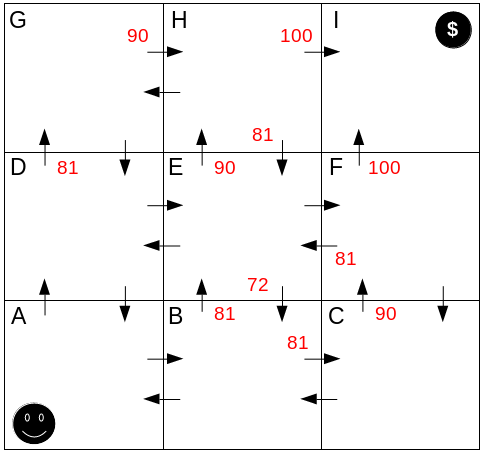
\includegraphics[width=0.44\textwidth]{img/exemplo-moeda-q-learning-4}
	\caption{Cenário da moeda com uma situação intermediária na execução do algoritmo}
	\label{fig:exemplo-moeda-q-learning-4}
\end{figure}

Ao final, desde que o número de episódios seja suficientemente grande, o algoritmo converge para a política ótima. Ou seja, a tabela $\widehat{Q}$ possui os valores de recompensa que fazem com que o agente siga a melhor sequência de ações possível. A Figura~\ref{fig:exemplo-moeda-q-learning-5} apresenta os valores de recompensa ao final da execução do algoritmo. Perceba que se o agente escolher a melhor ação de cada estado, ele chega ao destino com o menor número possível de passos. Perceba ainda que existem diferentes caminhos com o mesmo custo.

\begin{figure}[h]
	\centering
	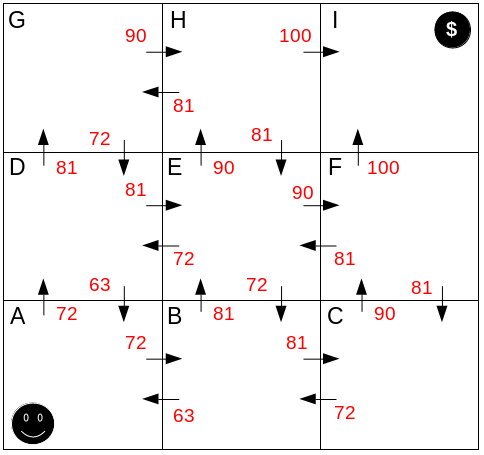
\includegraphics[width=0.44\textwidth]{img/exemplo-moeda-q-learning-5}
	\caption{Cenário da moeda ao finalizar a execução do algoritmo}
	\label{fig:exemplo-moeda-q-learning-5}
\end{figure}

Conforme discutido, a implementação de $\widehat{Q}$ geralmente é feita utilizando uma tabela com os estados $s \in S$ e as ações $a \in A$. A Tabela~\ref{tab:exemplo-moeda-q-learning} apresenta um exemplo de tabela $\widehat{Q}$ com os valores referentes ao estado intermediário apresentado na Figura~\ref{fig:exemplo-moeda-q-learning-4}. Para cada estado, o valor de recompensa esperada para cada ação é armazenado. Células com o caractere ``-'' indicam que não é possível realizar a respectiva ação no estado correspondente.

\begin{table}[h]
	\centering
	\begin{tabular}{r|ccccccccc}
		\multicolumn{1}{l|}{} & \textbf{A} & \textbf{B} & \textbf{C} & \textbf{D} & \textbf{E} & \textbf{F} & \textbf{G} & \textbf{H} & \textbf{I} \\ \hline
		\textbf{cima}         & 0          & 81         & 90         & 81         & 90         & 100        & -          & -          & -          \\
		\textbf{baixo}        & -          & -          & -          & 0          & 72         & 0          & 0          & 81         & -          \\
		\textbf{esquerda}     & -          & 0          & 0          & -          & 0          & 81         & -          & 0          & -          \\
		\textbf{direita}      & 0          & 81         & -          & 0          & 0          & -          & 90         & 100        & -         
	\end{tabular}
	\caption{Exemplo de tabela $\widehat{Q}$, representando a situação da Figura~\ref{fig:exemplo-moeda-q-learning-4}}
	\label{tab:exemplo-moeda-q-learning}
\end{table}

\clearpage

\section{Exercícios}

\resetexercisenumbering

\begin{exercise}
Mostre outras políticas ótimas para o ambiente em grade apresentado na Figura~\ref{fig:exemplo-rl-politica-otima}.
\end{exercise}

\begin{exercise}
Considere o cenário em grade apresentado abaixo com o estado objetivo de absorção \texttt{G}. A recompensa imediata é 10 para as transições rotuladas, e 0 para todas as demais.
\begin{enumerate}[a.]
	\item Apresente o valor de $V^*$ para cada estado do cenário. Apresente o valor de $Q(s, a)$ para cada transição. Finalmente, apresente uma política ótima. Use $\gamma = 0.8$.
	
	\item Sugira uma alteração na função de recompensa $r(s, a)$ que altera os valores de $Q(s, a)$, mas não altera a política ótima. Sugira uma mudança em $r(s, a)$ que altere $Q(s, a)$, mas não altere $V^*(s, a)$.
	
	\item Considere aplicar o algoritmo de $Q$-Learning no cenário em grade, assumindo que a tabela $\widehat{Q}$ é inicializada com zero. Assuma que o agente inicie na célula inferior esquerda e viaje no sentido horário ao redor do perímetro da grade, até encontrar o estado objetivo, completando o primeiro episódio. Descreva quais valores de $\widehat{Q}$ são modificados como resultado do episódio, e apresente seus valores atualizados. Responda à questão novamente, assumindo que o agente realize um episódio idêntico. Responda novamente para um terceiro episódio.
\end{enumerate}

\begin{figure}[h]
	\centering
	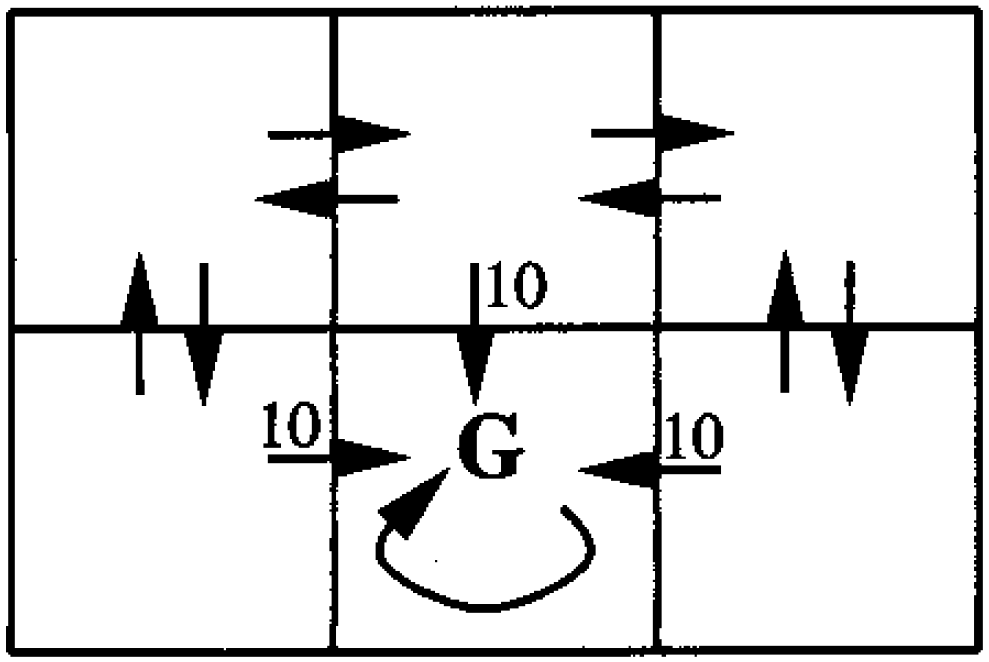
\includegraphics[width=0.25\textwidth]{img/exercicios/grade-rl}
\end{figure}
\end{exercise}

\begin{exercise}
O problema do penhasco é definido da seguinte forma:
\begin{itemize}
	\item Um robô está em uma sala mapeada como uma grade, conforme figura abaixo, onde seu objetivo é encontrar a saída. A posição inicial do robô é apresentada em verde, enquanto a porta é representada em azul. As células em vermelho compõem o penhasco. Logo, o robô deve aprender o menor caminho até a porta, sem que caia no penhasco.
	
	\item Os movimentos possíveis são \textit{cima}, \textit{baixo}, \textit{esquerda} e \textit{direita} (\textit{c}, \textit{b}, \textit{e}, \textit{d}).
	
	\item Ações que levariam o agente para fora da grade o deixam no mesmo lugar.
	
	\item Qualquer transição produz retorno imediato de -1, com exceção das que levam a estados do penhasco, que têm valor -100 e levam o agente de volta ao estado inicial.
\end{itemize}

\begin{figure}
	\centering
	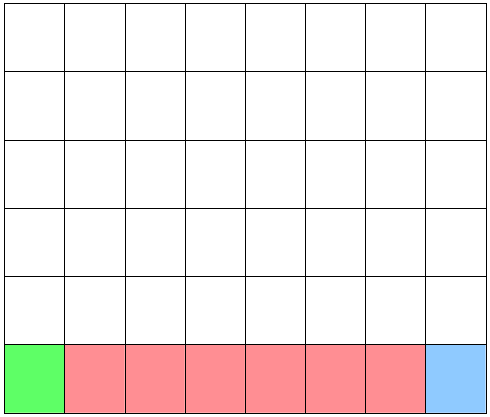
\includegraphics[width=0.5\textwidth]{img/exercicios/problema-penhasco}
\end{figure}

Com base nisso, implemente o algoritmo de $Q$-Learning para fazer com que o agente aprenda a sair da sala. Implemente uma interface para que o usuário possa informar os parâmetros do algoritmo, conforme abaixo:
\begin{itemize}
	\item Número de episódios.
	\item Estratégia de seleção da ação: \textit{guloso} ou \textit{$\epsilon$-guloso}.
	\item Valor de $\epsilon$.
\end{itemize}

Apresente os resultados, mostrando:
\begin{itemize}
	\item A tabela $\widehat{Q}$ resultante.
	\item A política ótima.
	\item Quantos episódios o algoritmo levou até a convergência.
	\item Qual o resultado de cada episódio.
	\item Comparação entre as diferentes estratégias de seleção da ação e os diferentes valores de $\epsilon$.
\end{itemize}

\end{exercise}
